\documentclass[acmsmall,nonacm]{acmart}
\usepackage{booktabs,amsmath,graphicx}
\setcitestyle{authoryear}
\settopmatter{printacmref=false,printccs=false}
\setcopyright{none}
\pagestyle{plain}
\renewcommand{\authorsaddresses}{}
\newcommand{\da}{\operatorname{DA}}
\title{More First Choices, Fewer Placements}
\subtitle{Shortlist design in New York rental simulations and Chilean school admissions}
\author{Ishan Khillan}
\affiliation{\institution{Harvard University}\city{Cambridge}\state{Massachusetts}\country{USA}}
\author{Elaine Zhang}
\affiliation{\institution{Harvard University}\city{Cambridge}\state{Massachusetts}\country{USA}}
\author{Todd Zhou}
\affiliation{\institution{Harvard University}\city{Cambridge}\state{Massachusetts}\country{USA}}
\renewcommand{\shortauthors}{Khillan, Zhang, and Zhou}
\begin{abstract}
A shortlist can improve its prediction of a family's offer while leaving another family without a place. We study this distinction in a simulation using New York rents and household budgets, and in four Chilean school admission cohorts with submitted lists and recorded offers. In Chile, adding rank to a frozen offer predictor put 5,552 more recorded offers on five-choice menus across 2,044,649 application records. Replaying deferred acceptance gave 2,218 more families their first choice and placed 1,787 fewer applicants overall. Of 2,527 people who lost a placement, 1,752 had unchanged menus. The rental simulations also produced more first choices and fewer placements. Neither comparison establishes a welfare ranking. We then ask how much prediction can improve if the entire tentative allocation must remain stable. Even allowing every eligible option and using the target in hindsight, the Chilean menus can cover at most 74 additional full-list partners under that requirement, compared with 5,975 under the unrestricted predictor switch. In the rental simulations there is room to improve coverage while protecting every recipient. In the three lottery cohorts tested, simulating competition without the realized tie order produced menus that beat the rank-informed predictor on historical coverage and placement at 64 draws, while assigning fewer first choices. The school offers used to score prediction are observed; placements under alternative menus in both settings are counterfactual.
\end{abstract}
\begin{document}
\maketitle
\section{Introduction}
Across four Chilean school admission cohorts, a five-choice shortlist that used an applicant's submitted rank was more likely to show the family its recorded offer. When we cleared all the new lists together, 2,218 more families got their first choice, yet 1,787 fewer applicants got a seat. Most people who lost a seat had exactly the same choices as before. That is 1.08 more first choices and 0.87 fewer placements per 1,000 application records. Looking only at the quality of each family's recommendations would miss what happened to its competitors. Looking only at the number placed would miss what families gained.

Why put school admissions next to apartment searches? We started with a practical question about rental advice: can the service uncover an affordable option that a household would otherwise miss? In our ordinary New York draws, 5,425 of 6,617 lower-income renter instances had no feasible listing in the first place. Asking rents and survey budgets let us distinguish lack of supply from limited consideration, and vary both supply and screening. They do not tell us who applied to an apartment or what offer they got. A similar pattern in school choice would matter for precisely that reason: in Chile we can replace the modeled order with families' own submitted rankings and score recommendations against offers the ministry actually recorded. And the comparison can fail. An entitlement outside the five choices changes who is protected, while the availability of affordable alternatives changes what a service can repair.

We compare the same first-five and random-five rules in both settings before evaluating the two site-specific recommenders. Both studies impose a binding display: a person can pursue only an option on their menu. The Chilean replay curates choices already reported; families did not face our five-choice rule. The rental replay uses centralized deferred acceptance to make competition explicit; New York landlords do not allocate apartments by that procedure. In both settings we ask what happens to other people when a platform decides which five options each applicant can pursue. Neither the magnitudes nor the housing assumptions are transferred across countries.

The policy question is what a service can change after tentative assignments are known. We give an exact test for switching whole lists, a bound on gross placement turnover when the test fails, and an exact calculation when the platform can replace individual options. It matters which changes the platform is allowed to make. Keeping all old offers supportable leaves considerable room to improve recommendations in the rental simulation, but almost none for predicting full-list partners in the Chilean cohorts. This is a limit on one concrete promise to applicants; it is not a claim that every better predictor must displace someone. In 2022--24 a rule using the full reports and 64 simulated priority draws beats the rank-informed predictor on both historical coverage and placement without seeing the realized tie order. The information available at the time of advice matters.
\section{What each experiment measures}\label{sec:design}
Let $E$ be the bipartite graph of acceptable applicant--program pairs. A displayed graph $D\subseteq E$ lists the programs an applicant can pursue. Each applicant strictly orders acceptable programs above being unplaced. A program has a fixed capacity and a strict priority ordering over applicants. It holds the highest-priority acceptable applicants who have proposed, up to its capacity. In the rental simulations each listing has one place. Let $M=\da(E)$ be the full-list allocation and $N_D=\da(D)$ the policy allocation; an unplaced applicant receives $\bot$. Stability means that no displayed pair would both prefer to match, taking account of vacancies and priorities. DA on a fixed graph is polynomial-time and applicant-optimal among its stable allocations \citep{gale1962,roth1986}.

For applicant $i$, define
\[
 C_i(D)=\mathbf{1}\{M(i)\ne\bot,\ (i,M(i))\in D\},\qquad
 P_i(D)=\mathbf{1}\{N_D(i)\ne\bot\}.
\]
Placement counts any acceptable assignment. It gives no extra credit for a first choice. Section~\ref{sec:ranks} measures rank separately. Both rates use all applicants. A person without a full-list partner contributes zero to coverage and can still receive a place after the lists change. In Chile we also compute $C_i$ using the historical offer instead of $M(i)$. For policies $A$ and $B$, the ordered pair $(C_i(B)-C_i(A),P_i(B)-P_i(A))$ belongs to a three-by-three table. The table identifies a person who newly sees their partner yet loses a placement. We use a separate indicator for exact equality of the two personal menus to identify people whose options stayed fixed while competitors' lists changed. Unchanged coverage by itself does not imply that a menu stayed fixed.

\begin{table}[ht]\centering\small
\caption{Two policy comparisons with a common allocation outcome. Each school application cycle is a separate national cohort.}\label{tab:design}
\begin{tabular}{@{}p{.19\linewidth}p{.35\linewidth}p{.37\linewidth}@{}}\toprule
& New York rentals & Chilean school admissions\\\midrule
Choices and priorities & Affordability and space rules, modeled tastes and screening & Submitted course rankings, published priorities and within-course tie orders\\
Shortlist change & Uniform five to Haiku five & Rank-blind predictor to rank-informed predictor, five discretionary choices plus entitlement\\
Reference option & Simulated full-list DA unit & Full-list replay program and recorded initial offer\\
Evidence & Archived model on development markets; first-five rule also tested on separate ads and households & Frozen 2019 models; four later cohorts for the specified signs\\
\bottomrule\end{tabular}
\end{table}

\paragraph{Relation to prior work.}
Competition between recommended options has a long history. \citet{rankings} optimize rankings jointly when job seekers apply and employers decide whom to interview. \citet{signals} study recommendations that reduce communication in matching markets. \citet{pruned} link unmatched hospitals under prefix truncation to missed stable partners. Our comparisons permit deletions anywhere on a submitted list and trace who is displaced. We use the classical invariance of matched participants on a fixed graph and results on entry and consistency \citep{galesoto,roth1986,crawford1991,sasaki}.

\citet{aguiarhong2026} compare stable and maximum assignments on restricted graphs and use Chilean school data to study retained rankings. We share their distinction between feasible and stable placements. We compare alternative fitted rules at a fixed quota and identify whose placement changes without a change in their own menu. \citet{smartplatforms} show in a field intervention that advice about admission risk can induce families to add options and improve actual placements. Here all comparisons hold the submitted reports fixed. \citet{munrointerference} studies how individual treatments spill over in designed markets, including Chilean school choice. We directly rerun specified menu policies on entire fixed cohorts and ask which changes preserve the original allocation. \citet{liu2024housing} audit the housing options language models recommend. Our housing exercise follows each recommendation through competition for a particular unit.

\subsection{What does showing a full-list partner guarantee?}\label{sec:two-theory}

The full-list partner in this section is an assignment in the same model as the restricted replay. The Chilean historical offer provides a separate empirical target.

\paragraph{The best prediction can send two people to one seat}
Three applicants share three one-seat programs $x,y,z$. The vector of first choices, in applicant order, takes the values $(x,y,z)$, $(x,z,y)$, $(y,x,z)$ and $(y,z,x)$ with probabilities $2/6,2/6,1/6,1/6$. Each state has distinct first choices, so all three receive those choices under full-list DA whatever the program priorities. The platform knows the probabilities but cannot see the state. With one slot per applicant, the unique choices maximizing expected partner coverage are $(x,z,z)$. They cover $5/3$ partners in expectation and place two people. The lists $(x,y,z)$ cover $3/2$ partners in expectation and place all three. Thus filling the third seat can cost as little as $1/6$ of an expected correct recommendation in this example.

\paragraph{What an omitted partner can explain}
Let $H$ be the applicants whose full-list assignment is a real program missing from $D$. Let $K_j$ and $T_j$ count members of $H$ assigned to $j$ under $M$ and $N_D$, respectively.
\begin{theorem}\label{thm:two-omission}
Relative to the full market, gross losses and gross gains in placement on $D$ are each at most $|H|-\sum_j\min(K_j,T_j)$. Furthermore, every unmatched applicant whose full-list partner is displayed can be paired with a distinct member of $H$ who is placed on $D$ and strictly prefers their full-list partner. Both conclusions hold for arbitrary stable selections on the two graphs.
\end{theorem}
\begin{proof}
Delete $H$ together with the seats its members occupy in each assignment. Any remaining blocking pair would have blocked the original assignment. Restrict the residual full-market allocation to the residual display: every surviving contract is visible there, and removing other edges cannot create a block. The two residual allocations are thus stable on the same pairs, using capacities $c-K$ and $c-T$, where $c$ is the original capacity vector. For fixed pairs, adding one seat retains every matched applicant and adds at most one: regard seats as unit copies with common order within each program, run seat-proposing DA, and admit the new proposer last. An applicant who holds an offer can only trade up. Matched-set invariance transfers this comparison to any stable selection \citep{galesoto,roth1986,crawford1991}. Comparing the two capacity vectors through their coordinatewise minimum bounds losses among the remaining applicants by $\sum_j(T_j-K_j)_+$ and gains by $\sum_j(K_j-T_j)_+$. Exactly $|H|-\sum_jT_j$ of $H$ lose a place, and none gain. Adding gives the bounds.

For the individual claim, at each program cancel the holders common to both assignments. Pair departing holders with incoming holders one-to-one until one side is exhausted. Start with an applicant who is unmatched on $D$ despite seeing their full-list partner $j$. Program $j$ must be full in $N_D$, and every new holder there outranks this applicant. Follow the pairing at $j$ to one of its new holders $h$. Full-list stability implies that $h$ had an assignment strictly preferred to $j$, since $j$ previously held a lower-priority applicant. If $h$ still sees that former assignment, repeat. Each step starts with someone who strictly prefers their former assignment and each pairing is injective. On a continued step the program is full after restriction. Its intake of new holders is therefore at least its number of departing holders, so the departing applicant always has a successor. The starting applicant has no incoming link, so the paths cannot cycle or meet. Each path ends at a placed applicant whose former assignment is hidden.
\end{proof}

For two policies $A,B$, one entry in the empirical comparison counts applicants with $C_i(B)-C_i(A)=1$ and $P_i(B)-P_i(A)=-1$. The theorem gives each such applicant a distinct other person on the final display who is assigned a worse program than their full-list partner, which is hidden under $B$. That other applicant can have the same list under $A$ and $B$. It can happen with only two applicants and one slot each. Let $i$ prefer $x$ to $y$, let $h$ prefer $y$ to $x$, and let both programs give $h$ higher priority. Full-list partners are $x$ for $i$ and $y$ for $h$. Display $A$ offers $i$ only $y$ and $h$ only $x$. Both place. Change only $i$'s list to $x$. Now $i$ sees their full-list partner and loses the competition for it. Under one-slot lists every witness is this direct: a new holder at the focal program could not also see their own strictly preferred full-list partner. The traced links in a larger market describe the two assignments and need not follow the chronology of DA proposals.

Let $p_{ij}(X)$ be the probability that $j$ is the full-list partner of $i$, given the information $X$ used to choose the lists. If a policy also uses randomness independent of the full allocation conditional on $X$, condition on its seed as well. By linearity, the conditional expected number covered is $\sum_i\sum_{j\in D(i)}p_{ij}(X)$. Selecting the most probable partners separately for each person therefore minimizes expected omissions, the coarse upper bound $|H|$ above. A smaller upper bound can coexist with fewer actual placements. For comparison, \citet[Theorem~4.7]{pruned} identify which hospitals can become unmatched under one-sided prefix pruning. Here omissions can occur anywhere in an incomplete list, and a displaced person can still see their own full-list partner.

\section{The same five-choice rule in both markets}\label{sec:common}
The two fitted recommenders use different inputs. A common benchmark lets us ask the same question in both settings. Suppose each person can list five options. What happens if everyone lists their five favorites? The alternative is to sample up to five feasible options uniformly without replacement for each applicant. In either case applicants propose in their original order. We keep any protected school entitlement outside the five slots. An applicant with at most five discretionary options sees them all. The benchmark uses modeled preferences in housing and families' submitted rankings in school choice. It tests what concentrating choices near the top of people's rankings can do at fixed capacity. The rental language model does not observe those realized rankings.

\begin{table}[ht]\centering\small
\caption{First five minus uniform five. Both outcomes use all applicants as the denominator. Changes are percentage points. NYC rates use the study's geographic weights. School rates give each application record equal weight.}\label{tab:common}
\begin{tabular}{@{}lrrr@{}}\toprule
Panel & Applicant instances & Full-list partner shown & Placed\\\midrule
NYC ordinary & 15,360 & $+21.03$ & $-13.86$\\
NYC enriched & 15,360 & $+17.03$ & $-18.88$\\
Chile 2022 & 570,891 & $+0.82$ & $-0.23$\\
Chile 2023 & 536,353 & $+0.99$ & $-0.23$\\\bottomrule
\end{tabular}
\end{table}

Choosing favorites raised full-list partner coverage and lowered placement in all four panels. To compute expected rental coverage under sampling, each full-list recipient with degree $d$ contributes $\min(5,d)/d$. Placement requires running DA. We averaged 48 uniform draws per market; Monte Carlo standard errors on the estimated placement rates were at most 0.022 percentage points in NYC and 0.0012 in Chile. These standard errors describe the numerical uncertainty in averaging menus. They do not measure uncertainty about the housing behavioral assumptions or about future cohorts. Short lists and continuity protections in Chile mean that many pupils receive exactly the same choices under either rule. The larger rental differences do not show that a housing recommender is intrinsically more harmful. The shared direction shows that the reversal can arise under a common rule in both settings. The school and rental policy comparisons use the same placement measure.

\paragraph{When keeping a favorite protects its recipient}
There is a precise reason to distinguish the school entitlement from an ordinary five-choice cap. If every list is a prefix of the applicant's full order, an applicant whose full-list DA partner survives that cut is placed at that program or one they prefer. To see this, run applicant-proposing DA on the prefixes, pausing anyone who exhausts their prefix. Continue that same run with the omitted suffixes restored. Those already holding an offer can only keep it or propose farther down their lists. Someone unplaced at the pause has already had every prefix option rejected. Order independence of DA gives the full-list allocation at the end \citep{gale1962,galesoto}. This is consistent with fewer placements relative to random menus: the guarantee concerns people whose full-list partner the prefix retains.

In the two rental designs every one of the 4,531 and 4,274 covered full-list recipients was indeed placed under first-five menus. In Chile an entitlement kept below the first five can break the prefix property. If an applicant ends up with a worse program while their full-list partner is hidden, their assignment must be one of those retained entitlements: a displayed top-five option could not be worse than an omitted one. The distinct witnesses from Theorem~\ref{thm:two-omission} must therefore end at such a returning pupil. We verified this for all 126 covered-but-unplaced applicants in 2022 and all 120 in 2023. The school institution supplies a concrete boundary of the guarantee.

\paragraph{Changing the rental ads and households}
We repeated the shared first-five comparison using separate survey donors and catalogues, without querying the language model. Among 8,400 supported markets, first-five increased partner coverage and reduced placement in both inventory designs in both evaluation windows. In September--October 2026 the ordinary-market changes were $+20.66$ and $-15.26$ percentage points, and the enriched-market changes were $+17.62$ and $-20.04$. In June--August 2025 the respective pairs were $(+20.05,-15.30)$ and $(+18.23,-18.92)$. The later enriched comparison covers only 79.97\% of the intended borough--month weight: Staten Island lacked supply and September Manhattan had only 29 eligible low-price ads for 32 required draws. The other three panels cover 97.95\%. Rates are normalized to the supported cells within each panel. These conditional simulations test the shared benchmark on different inventory and households. The Haiku comparison remains a development result.

\section{New York City rentals}\label{sec:twonyc}
We paired archived model recommendations with a simulation of who could rent each apartment. The inputs are recent-mover household records from the 2020--24 American Community Survey and rental advertisements first listed in June--August 2026 \citep{acs,firstmover}. Each market contains 64 renter instances and 64 available apartments from one borough and month. An apartment must meet bedroom needs and cost at most 40\% of monthly income. Lower-income households earn at most the survey-weighted median for NYC cash renters. Renter preferences combine rent, size, physical features, distance and taste shocks. Listing priorities depend on income relative to rent and a random shock specific to the renter--listing pair. We rerun applicant-proposing DA with exactly the same households, apartments and preferences under each display. The resulting placements are simulated. The ads provide asking rents, and the survey describes renter households. Neither source observes offers or leases between these parties.

In the ordinary design we sample households using survey weights and draw available apartments uniformly. In the enriched design half the inventory comes from a borough-specific affordability band. We then sample 32 lower-income households with a feasible option in that inventory and 32 higher-income households. This deliberate change lets us examine competition where lower-income households can participate. Each design has 20 seed blocks across three months and four supported boroughs, giving 240 paired markets and 15,360 renter instances. Staten Island had too few listings for draws of 64. The supported boroughs represent 97.95\% of the intended recent-mover geographic weight.

The income cutoff is \$64,435 in 2024 dollars. In asking-rent dollars at the study's July 2026 price base, the highest monthly rent allowed at the cutoff is \$2,286. We use the calibrated preference specification from the rental pilot. It selects a rent coefficient of 4 and an idiosyncratic shock scale of 0.5 from a nine-point grid. Its burden calibration has an observable limitation. At 217 lower-income placements across the 240 ordinary calibration markets, even a feasible assignment chosen to minimize their first-quartile rent burden cannot push that quartile below 27.78\%. The target quartile from recent movers' contract rents was 22.00\%. These finite-market bounds concern the calibration exercise. The household survey does not validate the assumed listing priorities or individual rankings.

\paragraph{What the recommender sees.}
For each renter, the five-slot uniform rule draws from the feasible listings without replacement. The archived Claude Haiku 5.5 recommender receives the same candidate set, a budget, bedroom needs, target area, prices, physical features and distances. The prompt asks it to choose five listings. It has no observations of other renters' menus or the realized preferences. Both policies show all feasible options to anyone with five or fewer. We used the 20,740 saved valid responses from the development pilot. Households and apartments can recur across draws. Rates below pool individual indicators within each borough-month and then average cells with equal month weights and Census recent-mover borough weights. The pointwise intervals resample entire paired seed blocks 10,000 times. They condition on the catalogues, behavioral model and stored replies.

\begin{table}[t]
\caption{NYC. Change under Haiku relative to uniform five-listing menus, in percentage points, with paired 95\% simulation intervals. Both columns use every renter in the row. A renter without a full-list DA partner contributes zero to partner coverage in both policies.}
\label{tab:nyc-two}
\centering\small
\begin{tabular}{llrr}
\toprule
Design & Renters & Full-list partner shown & Placed by DA\\
\midrule
Ordinary & All & $+5.62$ [$4.96,6.27$] & $-2.71$ [$-3.19,-2.23$]\\
 & Lower income & $+0.11$ [$0.00,0.24$] & $+0.00$ [$-0.19,0.21$]\\
 & Higher income & $+9.17$ [$7.99,10.34$] & $-4.58$ [$-5.27,-3.86$]\\
Enriched & All & $+5.85$ [$5.04,6.60$] & $-5.40$ [$-6.05,-4.73$]\\
 & Lower income & $+0.78$ [$0.19,1.43$] & $-0.92$ [$-2.23,0.37$]\\
 & Higher income & $+10.92$ [$9.47,12.29$] & $-9.88$ [$-10.43,-9.36$]\\
\bottomrule
\end{tabular}
\end{table}

\paragraph{What changed when everyone used the model?}
Under the original pilot design the primary endpoint was the lower-minus-higher difference in hidden blocking pairs. The comparison here follows the same people and uses the saved menus. Ordinary markets placed 53.89\% of renters under uniform lists and 51.18\% under Haiku, even as full-list partner coverage rose from 9.42\% to 15.04\% (Table~\ref{tab:nyc-two}). The direction depends on the comparator. Against a fixed score that ranks eligible apartments using their observable features, Haiku placed 20.26 points more renters in ordinary markets and 24.47 points more in enriched markets. Its coverage differences were $-0.44$ and $+0.66$ points, respectively.

\paragraph{What the group averages conceal.}
In the ordinary design, 5,425 of 6,617 lower-income renter instances had no feasible listing. The standardized change in their placement rate was smaller than one hundredth of a point. In enriched markets the change was $-0.92$ points with an interval spanning zero, yet 1,203 lower-income instances lost a placement and 1,044 gained one. The enriched lower-income share with a hidden blocking pair (a renter and an unshown apartment that each prefer the other to their assignment) rose from 37.03\% to 41.31\%. The higher-income share fell from 85.19\% to 78.01\%. The absolute gap narrowed even as hidden blocking pairs became more common for the lower-income group. Partner coverage and placement were secondary outcomes in this development pilot. We treat these results as evidence of a mechanism under specified assumptions.

\section{Chilean school admissions}\label{sec:chile}
The Chilean school choice system records the courses a family ranks, the school's priority and lottery information, and the initial offer the family actually receives \citep{saedata,correaschool}. We can ask whether a hypothetical shortlist would have included that offer. To learn who would receive a place on the new lists, we must replay the allocation.

We fitted two ridge logistic offer predictors to the same 483,070 applicants in 2019, using eligible discretionary applicant--course edges as observations. Both use program demand, capacity, congestion, list length, grade, priority indicators and a smoothed program offer rate estimated from 2019 (leave-one-out for training). The second adds log rank, a first-choice indicator and a rank--congestion interaction. We call the first score rank-blind because it omits these features. Both pipelines use rank to truncate at the continuity entitlement and to order proposals. Both break equal fitted scores with the same seeded edge-specific random keys. The 2019 fit uses observed offers as training labels; no evaluation-year offer enters either policy. Evaluation-year demand is computed from the entire submitted list profile. A platform could use this score after reports are collected; advance advice would require a demand forecast. The lottery is used for allocation only. Each predictor retains up to five discretionary choices. A pupil's guaranteed current-school option remains available outside that quota. The eligible graph retains the report down to this entitlement, including the entitlement itself. In the sequel a full-list partner refers to DA on these eligible regular-round entries. The selected courses keep their submitted order when applicants propose. We use the same priority tiers, published within-course order and pooled capacities for both replays. For course $j$, the main seat count is $\max(v_j,h_j)$, where $v_j$ is the published vacancy count and $h_j$ the number of eligible continuing applicants. The latter adjustment makes every protected return feasible. Neither input uses evaluation-year offers. Full-list DA reproduces the recorded program or outside option for 95.38\% of applicants in 2022 and 95.78\% in 2023.

\paragraph{The first confirmation and its extension}
After examining the 2020 and 2021 application years, we recorded a joint prediction before obtaining the 2022 and 2023 releases. These application years correspond to school entry in 2023 and 2024. The cohorts include 520,420 and 492,888 initial offer recipients, respectively. All applicants enter the placement and joint-transition counts. Giving the 2019 predictor access to rank would cover more historical initial offers and reduce replayed placements in each subsequent cohort. Table~\ref{tab:chile-frozen} reports both outcomes, with full-list DA partners as a second, directly comparable coverage target. Among the 2,493 net additional historical offers covered in 2022--23, 2,244 were offers that families explicitly accepted. The historical record does not tell us whether they would have accepted under either new policy.

Before downloading either of the next two releases, we committed the five-slot comparison, the two directional criteria and the inclusion of both 2024 and 2025 application years. We applied the same 2019 coefficients, 2019 program frequencies, quota, capacity adjustments and priority ordering without refitting. The original models passed both criteria in each additional year. Across these two new cohorts of 937,405 application records the rank-informed predictor covered 3,059 more recorded offers and placed 802 fewer applicants. Among the 1,072 who lost a placement, 748 had identical personal menus under both policies. Full-list replay agreed with the recorded program or outside option for 96.59\% in 2024 and 96.51\% in 2025. We reproduced every pupil's assignment with two implementations of DA under both policies and full lists. The fixed-priority model uses the within-course order in each release. For school entry in 2026 (application year 2025), the ministry replaced a random tie-break with a deterministic applicant--school ordering; the published field still supplies the realized order \citep{newtie,saedata}.

\begin{table}[ht]\centering\small
\caption{Rank-informed minus rank-blind school menus. Placement and full-list DA coverage come from the replay. Historical offer coverage uses the recorded initial course. Each entry is a net count in the same application-year cohort.}
\label{tab:chile-frozen}
\begin{tabular}{@{}lrrrr@{}}\toprule
Year & Applicants & Historical offers shown & Full-list partners shown & Placements\\\midrule
2022 & 570,891 & $+1,143$ & $+1,261$ & $-468$\\
2023 & 536,353 & $+1,350$ & $+1,473$ & $-517$\\
2024 & 473,482 & $+1,735$ & $+1,841$ & $-481$\\
2025 & 463,923 & $+1,324$ & $+1,400$ & $-321$\\\bottomrule
\end{tabular}
\end{table}

The choice of comparison matters. In the 2022 and 2023 cohorts we also reran DA on 48 uniform five-choice displays in each cohort and on the family's first five choices. Relative to the uniform-draw mean, the rank-informed policy covered about 9,235 and 9,740 more full-list partners and placed about 789 and 759 more pupils in 2022 and 2023. Relative to first-five, it placed 2,123 and 2,013 more. The rank-blind predictor placed the most pupils of these four policies in both years. Prioritizing predicted offers improved on simple lists, and adding rank information then moved the two outcomes in opposite directions.


\paragraph{A market-wide predictor}
Across 2022--24, a rule using the completed applications to simulate unknown priority draws covered more historical offers and placed more pupils than the rank-informed predictor in every 64-draw batch. The placement advantage was small, from 2 to 56 pupils per batch, and each batch gave fewer first choices. When compared with the rank-blind rule it still placed fewer applicants. Appendix~\ref{sec:school-sensitivity} gives the information available to the simulated rule, its tie handling, and the results at smaller simulation budgets. It also reports seat, quota and priority-order sensitivities. Under a larger seat convention the replay fits the recorded assignment less well, although the original policy comparisons retain their signs.

\section{A first choice and a place are different outcomes}\label{sec:ranks}
Was the lower placement count the price of better assignments for other applicants? To find out, we ranked each assignment on the person's original list, before either shortlist was made. A renter's order is modeled. For a pupil we use the rank the family entered, distinguishing the ministry's appended continuity option. An unplaced person stays in the denominator at every cutoff. Conditioning on being matched would omit the very people whose losses we want to measure.

\begin{table}[ht]\centering\small
\caption{Change in assignments at or above each rank. NYC compares Haiku with uniform menus, in geographically weighted percentage points. Chile compares the rank-informed predictor with the rank-blind predictor, in pupils. The first three school columns count only family-entered choices; the last includes any assignment, including an administrative fallback.}\label{tab:ranks}
\begin{tabular}{@{}lrrrr@{}}\toprule
 & First choice & Top three & Top five & Any placement\\\midrule
NYC ordinary (pp) & $+2.00$ & $+4.22$ & $+4.99$ & $-2.71$\\
NYC enriched (pp) & $+2.87$ & $+6.69$ & $+7.72$ & $-5.40$\\\addlinespace
Chile 2022 (pupils) & $+385$ & $+70$ & $-184$ & $-468$\\
Chile 2023 & $+515$ & $+116$ & $-181$ & $-517$\\
Chile 2024 & $+747$ & $+14$ & $-303$ & $-481$\\
Chile 2025 & $+571$ & $-38$ & $-254$ & $-321$\\\bottomrule
\end{tabular}
\end{table}

In every panel the new policy produces more first choices and fewer placements. Neither policy therefore dominates the other at every rank cutoff, in the sense of \citet{featherstone}. This conclusion also holds if we include each administrative fallback at its final list position: the first-choice and any-placement differences are unchanged. In the ordinary and enriched NYC markets, the paired 95\% simulation intervals for the first-choice gains are $[1.67,2.33]$ and $[2.41,3.32]$ percentage points. These are ranks on the modeled full order, not evidence that particular renters would have signed a lease.

There is precedent for this pattern under a different policy. In Chilean simulations \citet[Table~6]{correaschool} found that changing from course-specific lotteries to a common lottery increased both first choices and nonassignment. \citet{trace2026} also compare tie rules using several welfare measures. Our counterfactual keeps the priority order and quota fixed, changes the predicted shortlist, and observes which affected families had the same list under both policies.

A simple accounting exercise puts a price on the disagreement without estimating anyone's utility. Give one point for any placement and an additional $\lambda$ points for a first choice. On the four school cohorts together, the change in this index is $-1{,}787+2{,}218\lambda$. Someone using this objective would prefer the rank-informed rule if and only if $\lambda>1{,}787/2{,}218\simeq0.806$, with a tie at equality. Nothing in the data identifies that bonus or implies it is the same for all families. Counting assignments alone implicitly sets it to zero.

Who moved up? Ordering the outside option last and an appended continuity option after all family-entered choices, 8,076 Chilean applicants with edited lists got a strictly better result and 2,200 got a worse one. Among applicants with identical lists, 2,254 improved and 7,215 worsened. Each of the four years has this same split in direction. These are paired changes between two full-market replays. The two groups differ in list length and exposure to competition. Comparing their rates would not identify a treatment effect of editing one's own list.

\section{Who loses a placement?}\label{sec:who}
At the level of a whole market, both studies give instances of higher coverage and fewer placements. The losses reach different people. Figure~\ref{fig:losses} partitions everyone who was placed under $A$ and unplaced under $B$. We first separate people whose menu was identical. Among the rest, we ask whether their full-list partner became visible, became hidden, or had the same visibility as before.

\begin{figure}[ht]
\centering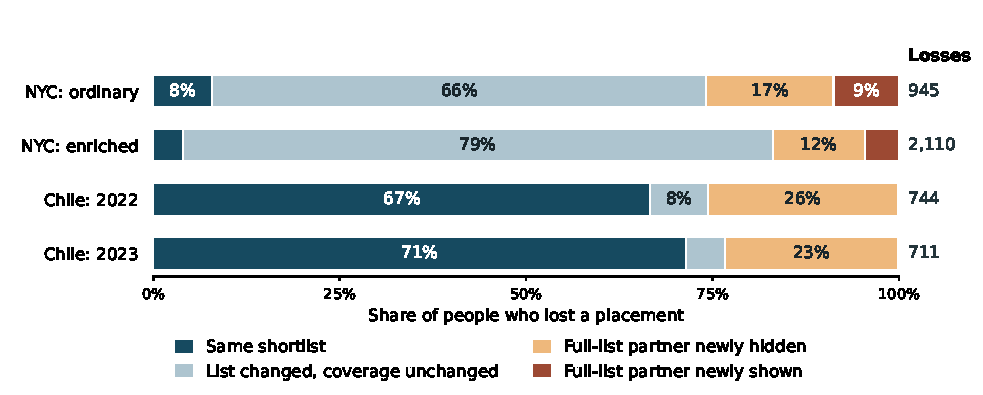
\includegraphics[width=.97\linewidth]{figures/placement-losses.pdf}
\caption{What changed for people who lost a placement? Bars within each row sum to 100\%. Numbers at right are raw gross losses. A changed list can retain the same partner coverage, including when the applicant had no full-list partner. The latter applicants still count in the analysis.}
\Description{The share of placement losses on an identical menu is small in the rental simulation, and about seven in ten in both Chilean school cohorts.}
\label{fig:losses}
\end{figure}

\paragraph{A change that reaches someone else's list.}
In the original 2022--23 Chilean cohorts, only 32,914 of 1,107,244 application records had different displayed courses under the two predictors. Of 1,455 applicants who lost a placement, 1,004 had exactly the same personal menu. The reverse happened to 406 of the 470 who gained one. Holding preferences, priorities, capacities and an applicant's own list fixed, a change in that applicant's placement can arise only through competitors' menus. These spillovers account for a net loss of 598 seats among applicants whose lists stayed fixed. Among the 32,914 applicants with edited lists, 451 lost a place (1.37\%). Among the 1,074,330 with identical lists, the 1,004 losses represent 0.093\%.

In the ordinary NYC markets, 945 renter instances lost a placement and 475 gained one. Of the 945 who lost, 74 saw identical menus and 83 newly saw their full-list partner. In enriched markets, 2,110 lost a placement and 1,212 gained one. Here 83 of those who lost saw identical menus and 97 newly saw their partner. Over both designs, newly seeing one's full-list partner and losing a place happened to 180 renter instances. For all 180 we found the distinct displaced-partner witnesses in Theorem~\ref{thm:two-omission} within their respective market. Of these paths 169 reached a witness after one program. Longer paths involved up to three programs.

\paragraph{The newly shown school offer often converted.}
In Chile in 2022--23, 3,750 applicants newly saw their full-list DA partner under the rank-informed predictor. Of these, 3,728 obtained that exact course in the replay and 20 obtained a different course. The remaining two went unplaced. In ordinary NYC markets 1,056 of the 1,720 newly shown renters obtained the named apartment (61.4\%); in enriched markets it was 1,277 of 2,012 (63.5\%). Across all applicants in each NYC design the number receiving their exact full-list partner increased by 523 and 553, respectively. Across the two school cohorts it increased by 5,049. More people therefore received their exact full-list partner even while fewer received any placement. We verified both displacement paths. Analyzing the recorded historical offer as a separate target, 3,366 of the 3,622 applicants who newly saw that program received it in the replay. Thus a platform could document a high rate of placement at the newly shown program and still miss a loss elsewhere in the market. The witness theorem applies to the modeled full-list partner. It uses stability and cannot be applied to an arbitrary historical offer.

\paragraph{Feasibility and priorities.}
Let $\nu(D)$ be the largest number who can simultaneously take displayed options within capacity, and $g(D)=\nu(D)-|N_D|$ the feasible places unrealized by DA. The placement change is $\Delta\nu-\Delta g$ \citep{aguiarhong2026}. In ordinary NYC markets, displayed capacity fell by 3.84 percentage points and the shortfall shrank by 1.13, giving the observed 2.71-point decline. In enriched markets those changes were $-12.29$ and $-6.89$ points. The school results differ. In 2022 the display could accommodate 244 fewer applicants and the shortfall grew by 224, for a loss of 468. In 2023 those figures were 153 and 364, for a loss of 517. Each school maximum is certified by a feasible flow and a cut of equal value. This benchmark uses only displayed edges and seat counts. It relaxes priorities and the obligation to place a particular returning pupil. These identities describe two margins on the same graph. They do not isolate the causal effect of changing priorities.

\section{Changing lists while protecting tentative offers}\label{sec:row-screen}

Suppose the platform observes an allocation $M_A$ stable on the old lists before deciding who receives new lists. Both menus retain the same underlying ranking over programs. Each person can receive either their entire old row $A_i$ or their entire proposed row $B_i$. Flag row $i$ if either (i) $M_A(i)$ is a real program missing from $B_i$, or (ii) $B_i$ contains a pair $(i,j)$ that would block $M_A$. For the second test, $i$ must prefer $j$ to $M_A(i)$, and $j$ must have a vacancy or prefer $i$ to one of its holders. Since $M_A$ is stable on $A$, only newly added options need this test. Let $F$ be the flagged applicants. With indexed rankings, check feasibility of each old contract and compute each program's occupancy and worst incumbent priority once. A scan of the proposed edges then constructs $F$ in linear time in the explicit menu and capacity input size. This rule uses baseline assignments and the rankings relevant to these pairs. In a simulation it can use the modeled rankings; a service with incomplete information would need to elicit these comparisons.

\begin{theorem}\label{thm:two-policy-screen}
If $S$ receives its proposed rows, $M_A$ remains stable exactly when $S\cap F=\varnothing$. On any such display every stable outcome has the original recipients, and applicant-proposing DA weakly improves every applicant's assignment relative to $M_A$. For an additive row objective with gain $g_i$ from switching row $i$, the largest net gain that keeps $M_A$ stable is $\sum_{i\notin F}(g_i)_+$.

More generally, put $R=S\cap F$ and let $N$ be any stable outcome on the mixed display. Let $K_j$ and $T_j$ count people in $R$ assigned to program $j$ under $M_A$ and $N$, respectively. The gross numbers of placement losses and gains are each at most
\[
 \bigl|\{i\in R: M_A(i)\ne\bot\text{ or }N(i)\ne\bot\}\bigr|-\sum_j\min(K_j,T_j)\ \leq\ |R|.
\]
\end{theorem}
\begin{proof}
A removed baseline partner makes $M_A$ infeasible. A newly displayed blocker prevents its stability. Both defects depend only on the applicant's row when the allocation being tested is fixed. In their absence every old contract survives and every displayed pair passes the blocking test. Matched-set invariance and applicant optimality give the first guarantees. The objective is therefore maximized by switching precisely the unflagged rows with positive gain, with free choice on zero gains.

For the bound, remove $R$ and its occupied seats from both allocations. In $M_A$ all remaining assignments survive on the mixed display and no remaining pair blocks. In $N$ stability also survives the restriction. Compare the resulting capacity vectors $c-K$ and $c-T$ using the one-seat argument of Theorem~\ref{thm:two-omission}. Outside $R$, losses are at most $\sum_j(T_j-K_j)_+$ and gains are at most $\sum_j(K_j-T_j)_+$. Within $R$, losses equal $\sum_j K_j-d$ and gains equal $\sum_j T_j-d$, where $d$ counts members matched under both allocations. Adding either margin yields the stated expression.
\end{proof}
The condition protects the old allocation as a stable witness. A flagged applicant can still switch without causing any placement loss. The distinction allows the rule to be checked before reallocation and limits the gains it can deliver. For independent switches with probabilities $p_i$, the probability that the old allocation remains stable is $\prod_{i\in F}(1-p_i)$, and expected gross losses or gains are at most $\sum_{i\in F}p_i$. The probability factorization is related to the one-sided uncertainty result of \citet{aziz_uncertain}. Here program priorities stay fixed and applicant menus change.

For a fixed reference partner, $g_i=C_i(B)-C_i(A)$. Maximizing this objective using the partner's identity gives a hindsight ceiling. In the 2022--23 school cohorts, 27,851 of 32,914 changed rows could switch together while supporting every old contract. Only 22 of the 3,750 newly shown full-list partners occurred on those rows. A platform could reasonably object: why choose between two complete lists when it can replace just one option? We address that objection next. Appendix~\ref{sec:rollout} separately studies random partial adoption without protection.

\subsection{How much does changing one slot at a time buy?}\label{sec:slots}
Fix the same baseline assignment $M_A$. For applicant $i$, let $U_i$ be a candidate pool containing $A_i$, and let $q_i=|A_i|$ include any protected slots. The required set $L_i$ contains the applicant's baseline partner if matched and all policy-protected options (in Chile, the continuity course if entitled). Let $V_i$ consist of the options in $U_i$ that do not form a blocking pair with $i$ at $M_A$. Inspecting a pair requires the applicant's preference relative to the current assignment and the program's vacancy or priority cutoff at that assignment.

\begin{proposition}\label{prop:slots}
The menus with exactly $q_i$ options per applicant that respect entitlements and keep $M_A$ stable are precisely
\[
 L_i\subseteq D_i\subseteq V_i,\qquad |D_i|=q_i\quad\text{for every }i.
\]
For any additive edge score, an optimal such menu keeps $L_i$ and fills the remaining slots with the highest-scored options in $V_i\setminus L_i$. For a single known reference option per applicant, the exact coverage gain over baseline is the number of previously hidden reference options in $V_i$ whose applicant has a free slot $q_i>|L_i|$.
\end{proposition}
\begin{proof}
Removing a required partner makes $M_A$ infeasible; revealing any blocker makes it unstable. Conversely, if the required edges survive and no blocker is visible, $M_A$ is stable on the new display. This gives exactly the displayed family of sets. It is nonempty since the old list is feasible in every row. Exchanging a lower-scored optional edge for a higher-scored eligible one can only increase the objective. For the coverage claim, give each reference edge score one and break ties in favor of old options. Every old hit can be kept, and each admissible missing reference with room in its own row can be added independently.
\end{proof}
The blocking-pair test has a direct predecessor: \citet[Observation~1]{boehmer2021} show that deleting blocking edges suffices to stabilize a specified matching in one-to-one markets. Here the quantity of interest is how much of a proposed recommender's objective can be retained at a fixed quota, with institutional entitlements. As in Theorem~\ref{thm:two-policy-screen}, the original contracts form a stable witness. DA may select a different allocation, but every original recipient remains placed at a weakly preferred option and no previously unplaced applicant enters. The rule requires a known tentative assignment and the comparisons just described. It cannot be run from scores alone.

\begin{table}[ht]\centering\small
\caption{Additional full-list partners shown over the original menus. ``Whole'' and ``Slots'' are hindsight maxima under the stable-witness requirement. ``Score'' edits individual slots over all feasible options without seeing the target. ``Switch'' adopts the proposed policy without the requirement. Counts pool applicant instances within each setting.}\label{tab:slotrepair}
\begin{tabular}{@{}lrrrrr@{}}\toprule
 & Whole lists & Slots, $A\cup B$ & Slots, all & Score & Switch\\\midrule
NYC ordinary & 132 & 591 & 2,014 & $+243$ & $+867$\\
NYC enriched & 133 & 662 & 3,018 & $+193$ & $+912$\\
Chile 2022--25 & 44 & 51 & 74 & $+10$ & $+5,975$\\\bottomrule
\end{tabular}
\end{table}

Why is the school ceiling so low? Of 1,885,296 full-list partners in the four cohorts, the blind menus already showed all but 9,407. Of those misses, 9,333 would themselves block the old assignment if displayed. No amount of rearranging the other four slots can make those pairs compatible with that assignment. Every one of the remaining 74 can be added; the quota rules out none. The conclusion changes in the rental markets. Of 6,377 missing partners in the ordinary markets, 2,014 could still be shown, as could 3,018 of 8,728 in enriched markets. This is a difference in the composition of the missed targets, in addition to the much higher starting coverage in Chile.

The two benchmarks use different information. A clearinghouse that knows all inputs and tie orders can compute its own full-list DA target. A predicted historical offer and an apartment allocation under unobserved tastes are different objects. For the score column we instead maximize the frozen rank-informed school score, or the number of the rental model's proposed picks retained (the archive records selections, not scores for every listing). Neither uses the target. Under these edits DA retained the same people in every market and gave 67 and 80 renters a strictly better modeled assignment across the two designs. Across the four school cohorts, 12 pupils improved. For the separate historical-offer target, the score rule actually \emph{lost} 30 hits in Chile; the hindsight maximum was a gain of 645. The rule guarantees protection, not an improvement on an unknown prediction target. Nor is 74 an upper bound if contracts may move and the only requirement is retaining the same headcount.

\paragraph{Can a platform improve prediction and placement together?}
Yes in these cohorts, if it has more information. Consider a clearinghouse that already knows all reports, capacities and realized priority orders. Compute full-list DA, keep each matched applicant's full-list partner and any entitlement, then fill the other slots by the frozen rank-informed score. All full-list contracts remain feasible; restricting a stable display cannot create a blocking pair for that assignment. The full-list allocation is therefore stable on the new menus. The set of recipients stays the same as in full-list DA, although a person's exact partner can change. This construction fits the five discretionary slots because each applicant needs to retain at most one partner in addition to the entitlement.

Compared with the unrestricted rank-informed predictor, this rule showed \emph{more recorded historical offers} in every year ($+856,+814,+660,+489$) and also placed more pupils ($+42,+60,+39,+38$). It used no historical offer as input. This rules out an inherent prediction--placement frontier even for the observed target. The guarantee protects the full-list allocation, a different baseline from the rank-blind seats protected in Table~\ref{tab:slotrepair}. A service advising applicants before reports or tie orders exist cannot simply run this rule, and the housing ads do not supply the required preferences.

\section{Implications and limits}
A school platform looking only at recorded offers would endorse adding rank to its predictor. A platform looking only at placement would reject the same change. Neither verdict mentions the increase in first choices or identifies the people who bear the loss. The families whose menus changed tended to move up in the replay. Families with the same menu who moved at all tended to move down. It is possible to value first choices highly and still want to protect those applicants. The calculation in Section~\ref{sec:row-screen} shows exactly what protecting every old contract permits. Appendix~\ref{sec:remedy} considers a narrower intervention after offers: referring an unmatched person to a vacancy without taking anyone else's contract.

The rental experiment addresses a different social concern. A renter who cannot afford a single listing has zero hidden blocking pairs and zero chance of placement under either policy. A group can consequently score well on a hidden-options measure while having almost no access to housing. We keep these households in the denominator, report their feasible sets, and examine how much discretion the platform has once tentative offers exist. Giving lower-income renters priority among equally large referral assignments had room to move only three additional placements toward them in the ordinary draws. A service that also changes affordability or expands search would face a different feasible graph.

\paragraph{Limits of the evidence.}
The housing data identify asking rents and surveyed household characteristics. Preferences, housing-provider priorities, budgets and assignments are modeled. The budget in the prompt is correlated with income, even though group membership is absent from the prompt. The language-model result conditions on one model version and one saved response per queried renter. The independent catalog check evaluates only the first-five benchmark. The data contain no broker relationships or commissions, and the study does not identify steering. In Chile the rank-informed model already has access to families' ordered applications. Its evidence concerns curation of known choices. The actual admissions system uses reserves and family contingencies beyond the pooled-priority replay. Changing what a platform displays could change what people search for, how they report, who applies, or whether they accept. If a shortlist is merely advice and families can freely apply off-list, the assumed restriction need not bind. Neither study estimates those responses, preference intensity, or a causal effect of deployment. The baseline school replay disagrees with the official course or outside option for 3.4--4.6\% of records, much larger than the net placement change (about 0.07--0.10 percentage points by year). Restricting the \emph{accounting}, after clearing each entire cohort, to applicants whose full-list replay agreed with the historical outcome still gives net losses of 356, 400, 399 and 259. This locates the result; replay agreement for one person cannot establish that all competitors would behave as modeled. The Chilean application years may include some of the same children. We treat them as finite cohorts and report exact counts. The shared first-five benchmark uses the same rule in both settings. The site-specific recommenders address different decisions. We do not pool their effect sizes.

\paragraph{What a platform can audit.}
Record the available options and capacities, the two complete sets of proposed lists, the reference offer where one exists, and the assignment induced by each set of lists. Those records distinguish a successful recommendation to its intended recipient, a lost place on a list that never changed, and a person without any feasible alternative. The last case points to a constraint on supply. The first two call for evaluating recommendation and allocation together.


\paragraph{Reproducibility.}
The accompanying code regenerates the two studies' aggregate tables and figures. In NYC we checked 2,880 published market-by-group endpoint rows against the regenerated menus. The legacy reply cache stores listing indices without a digest of the original prompt payload. Its consistency with this reconstruction can be checked, while the exact original payload cannot be authenticated independently. In Chile we recomputed the blind, rank-informed and full-list assignments in the original two cohorts and checked all 3,321,732 applicant--policy outcomes against the archived serial solver. The 2022--23 sign criterion was recorded locally before data acquisition. The extension to 2024--25 was committed to the research repository before downloading either release. The joint transitions, alternative-baseline, rollout, sensitivity and referral analyses are follow-ups. The two additional cohorts yielded a further 2,812,215 person--policy checks. All shared school outputs are aggregates.

\paragraph{Use of AI.} The team used OpenAI Codex extensively in developing the mathematical arguments, implementing and checking the replays, and drafting and revising the manuscript. The Claude model used to select rental menus is part of the experiment, a separate use described in Section~\ref{sec:twonyc}.

\bibliographystyle{ACM-Reference-Format}
\bibliography{paper}
\clearpage
\appendix
\section{What changes during a partial rollout?}\label{sec:rollout}
A service might try the new rule on a fraction of applicants and use the result to judge a full switch. We simulated that decision on the original 480 rental markets and two school cohorts. Independently for each applicant, we use policy $B$'s full menu with probability $p$ and otherwise keep $A$'s. We clear the entire market at each $p\in\{0,1/4,1/2,3/4,1\}$. We use 64 independent pairs of random assignments, with complementary uniforms within a pair and shared draws across uptake levels. This design gives a Monte Carlo standard error conditional on the fixed cohorts, preferences and candidate menus. For NYC we also resample whole simulation seed blocks. These experiments were specified after the original full-switch comparisons.

For any fixed reference offer, the expected number of people shown that offer is exactly the interpolation between the two endpoint counts: menu membership depends only on that person's switch. At half adoption the complementary assignments give that midpoint exactly in each pair. Placement need not follow the same line. For example, if two one-slot menus both show $x$ before the switch and both show $y$ afterward, either endpoint places one applicant. A mixed market with one applicant at each site places two. Reversing two initially distinct menus can bend the placement curve in the opposite direction.

\begin{figure}[ht]
\centering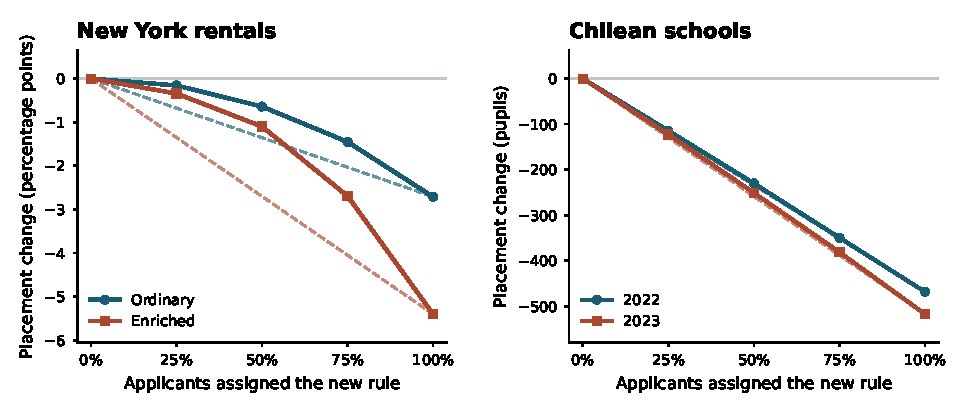
\includegraphics[width=.98\linewidth]{figures/adoption.pdf}
\caption{Placement change from the original policy when applicants independently switch to the proposed menu. Points give the simulated mean at each uptake. Dashed lines interpolate between full adoption and the original policy. The Chile panel reports pupils within each national cohort; the NYC panel uses geographically standardized percentage points.}
\Description{Placement declines in both markets. New York's mixed-policy outcomes sit above the straight-line interpolation by a larger proportion of the full-switch effect. The school curves lie close to their endpoint lines.}
\label{fig:uptake}\end{figure}

Placement at half adoption exceeded the interpolation by 0.71 and 1.60 percentage points in New York. The corresponding 95\% simulation-block intervals were $[0.59,0.84]$ and $[1.40,1.82]$, with Monte Carlo standard errors of 0.009 and 0.010 points. In Chile the midpoint deviation was about four pupils in 2022 and eight in 2023 (Monte Carlo standard errors 0.45 and 0.44 pupils, respectively). The school curves are close to linear in aggregate, yet applicants still change places. At half adoption an average of 272 pupils in 2022 and 271 in 2023 lost a place on a menu identical under both policies. The corresponding gains were 145 and 107. A nearly linear aggregate curve offers little protection to an individual family.

\section{Changing lists while protecting tentative offers}\label{sec:row-screen}

Suppose the platform observes an allocation $M_A$ stable on the old lists before deciding who receives new lists. Both menus retain the same underlying ranking over programs. Each person can receive either their entire old row $A_i$ or their entire proposed row $B_i$. Flag row $i$ if either (i) $M_A(i)$ is a real program missing from $B_i$, or (ii) $B_i$ contains a pair $(i,j)$ that would block $M_A$. For the second test, $i$ must prefer $j$ to $M_A(i)$, and $j$ must have a vacancy or prefer $i$ to one of its holders. Since $M_A$ is stable on $A$, only newly added options need this test. Let $F$ be the flagged applicants. With indexed rankings, check feasibility of each old contract and compute each program's occupancy and worst incumbent priority once. A scan of the proposed edges then constructs $F$ in linear time in the explicit menu and capacity input size. This rule uses baseline assignments and the rankings relevant to these pairs. In a simulation it can use the modeled rankings; a service with incomplete information would need to elicit these comparisons.

\begin{theorem}\label{thm:two-policy-screen}
If $S$ receives its proposed rows, $M_A$ remains stable exactly when $S\cap F=\varnothing$. On any such display every stable outcome has the original recipients, and applicant-proposing DA weakly improves every applicant's assignment relative to $M_A$. For an additive row objective with gain $g_i$ from switching row $i$, the largest net gain that keeps $M_A$ stable is $\sum_{i\notin F}(g_i)_+$.

More generally, put $R=S\cap F$ and let $N$ be any stable outcome on the mixed display. Let $K_j$ and $T_j$ count people in $R$ assigned to program $j$ under $M_A$ and $N$, respectively. The gross numbers of placement losses and gains are each at most
\[
 \bigl|\{i\in R: M_A(i)\ne\bot\text{ or }N(i)\ne\bot\}\bigr|-\sum_j\min(K_j,T_j)\ \leq\ |R|.
\]
\end{theorem}
\begin{proof}
A removed baseline partner makes $M_A$ infeasible. A newly displayed blocker prevents its stability. Both defects depend only on the applicant's row when the allocation being tested is fixed. In their absence every old contract survives and every displayed pair passes the blocking test. Matched-set invariance and applicant optimality give the first guarantees. The objective is therefore maximized by switching precisely the unflagged rows with positive gain, with free choice on zero gains.

For the bound, remove $R$ and its occupied seats from both allocations. In $M_A$ all remaining assignments survive on the mixed display and no remaining pair blocks. In $N$ stability also survives the restriction. Compare the resulting capacity vectors $c-K$ and $c-T$ using the one-seat argument of Theorem~\ref{thm:two-omission}. Outside $R$, losses are at most $\sum_j(T_j-K_j)_+$ and gains are at most $\sum_j(K_j-T_j)_+$. Within $R$, losses equal $\sum_j K_j-d$ and gains equal $\sum_j T_j-d$, where $d$ counts members matched under both allocations. Adding either margin yields the stated expression.
\end{proof}
The condition protects the old allocation as a stable witness. A flagged applicant can still switch without causing any placement loss. The distinction allows the rule to be checked before reallocation and limits the gains it can deliver. For independent switches with probabilities $p_i$, the probability that the old allocation remains stable is $\prod_{i\in F}(1-p_i)$, and expected gross losses or gains are at most $\sum_{i\in F}p_i$. The probability factorization is related to the one-sided uncertainty result of \citet{aziz_uncertain}. Here program priorities stay fixed and applicant menus change.

For a fixed reference partner, $g_i=C_i(B)-C_i(A)$. Maximizing this objective using the partner's identity gives a hindsight ceiling. In the 2022--23 school cohorts, 27,851 of 32,914 changed rows could switch together while supporting every old contract. Only 22 of the 3,750 newly shown full-list partners occurred on those rows. A platform could reasonably object: why choose between two complete lists when it can replace just one option? We address that objection next. Appendix~\ref{sec:rollout} separately studies random partial adoption without protection.


\section{How many vacancies could one referral fill?}\label{sec:remedy}
With tentative offers in hand, could the platform fill a vacancy by referring one unmatched applicant to it? We consider only affordable, feasible apartments or eligible courses already on the original report. Each referral must preserve the existing contracts together in a stable allocation.
\subsection{One coordinated referral after offers}\label{sec:two-referral}

Suppose the platform now observes an assignment $M_0$ stable on the initial lists. Join each unmatched applicant to each mutually acceptable program with a current vacancy. These edges are hidden: if one were displayed it would block $M_0$. Give each program its remaining capacity and let $r$ be the size of a maximum matching in this graph. With lists of $\min(k,d_i)$ programs, where $k\ge1$ and $d_i$ is feasible degree, a hidden option can always replace a displayed one. If an entitlement is protected outside the quota, the substitution is made in a discretionary slot. In both replays, every selected applicant had a full five-slot discretionary list.

\begin{theorem}\label{thm:two-referral}
Among extensions that keep every initial contract in a single stable assignment, the maximum number of additional recipients is $r$. One shortlist substitution per selected applicant attains it. Every stable outcome on the revised display gives each consenting applicant their named referral, even if others decline. Under applicant-proposing DA, every original recipient also receives a weakly preferred assignment.
\end{theorem}
\begin{proof}
The new contracts in any extension must form a residual matching. Conversely, choose any such matching $A$. For each consenting participant substitute their assigned program for their last discretionary displayed option. Write $W$ for the original assignment together with the accepted referrals. All new pairs in the display belong to $W$. On old edges the applicant weakly improved. An originally full program has the same holders. At an originally slack one, every applicant with an old edge weakly preferred their original assignment, by stability. Hence $W$ is stable on this display. DA weakly dominates $W$ for applicants. All stable selections have the same matched people \citep{roth1986}. If some stable selection omitted an accepted referral $e$, it would keep its recipient matched even after deleting that unused edge. On that same graph $W\setminus\{e\}$ is stable by the preceding argument, since this applicant now has a subset of their original list. That would leave the person unmatched in one stable outcome only, a contradiction.
\end{proof}
The maximum fixes the original contracts in a stable witness. Opening new options to incumbents would be a different intervention. The empirical calculation also requires deciding which hidden options a person would actually accept. We report both a top-five rank limit and all mutually acceptable vacancies. Work on facilitating matches, adding school seats and guaranteed school referrals provides related interventions \citep{facilitate,tworound,lepesure}.


\begin{table}[ht]\centering\small
\caption{Largest number of named referrals compatible with retaining all existing contracts in one stable allocation. NYC uses simulated Haiku offers. Chile uses rank-informed pooled DA offers. All counts use instances in their own row. A vacancy must be at an affordable, feasible listing or an eligible course already on the pupil's reported list.}\label{tab:ref}
\begin{tabular}{@{}lrrrr@{}}\toprule
& Vacant seats & Unplaced with an option & Any rank & Top five\\\midrule
NYC ordinary & 7,972 & 757 & 683 & 204\\
NYC enriched & 5,990 & 2,527 & 1,926 & 370\\
Chile 2022 & 601,565 & 128 & 127 & 0\\
Chile 2023 & 640,751 & 97 & 97 & 1\\\bottomrule
\end{tabular}
\end{table}

In ordinary NYC markets only 37 unplaced lower-income renter instances could use any vacancy. Of the maximum 683 additional placements, at least 22 and at most 25 could go to them. In enriched markets 1,601 unplaced lower-income renters could use a vacancy. Maximizing total referrals first, then minimizing or maximizing referrals to this group, gave 1,002--1,085 lower-income recipients among 1,926 placements. Both supply and the households sampled change across these designs.

Many residual school seats were in courses that no unmatched pupil had listed. With full take-up, at most 224 placements could be added across the two years. Just one was possible within the family's top five. Neither year had an eligible referral after the rank-blind allocation, so even after each policy's largest extension the rank-informed policy placed 761 fewer pupils. After uniform rental menus the corresponding maxima were 215 ordinary and 518 enriched placements.

We verified the school maxima with a second national flow implementation. We replaced each selected applicant's last discretionary option with their referral, reran DA, and checked each named assignment, the weak improvement for earlier recipients, the quota and continuity rights. A service would need to observe current offers, elicit acceptable alternatives and give each family a chance to decline. Table~\ref{tab:ref} reports the opportunities available under those conditions.

\end{document}
